% Template for DAN, KLTN, SVNCKH 

\documentclass[oneside,a4paper,13pt]{extreport}
\setcounter{secnumdepth}{4}
\setcounter{tocdepth}{4}
% Font tiếng Việt
\usepackage[T5]{fontenc}
\usepackage[utf8]{inputenc}
\DeclareTextSymbolDefault{\DH}{T1}

% Tài liệu tham khảo
\usepackage[
	sorting=nty,
	backend=bibtex,
	defernumbers=true]{biblatex}
\usepackage[unicode]{hyperref} % Bookmark tiếng Việt
\addbibresource{References/references.bib}

\makeatletter
\def\blx@maxline{77}
\makeatother

% Chèn hình, các hình trong luận văn được để trong thư mục Images/
\usepackage{graphicx}
\graphicspath{ {images/} }

% Chèn và định dạng mã nguồn
\usepackage{listings}
\usepackage{color}
\definecolor{codegreen}{rgb}{0,0.6,0}
\definecolor{codegray}{rgb}{0.5,0.5,0.5}
\definecolor{codepurple}{rgb}{0.58,0,0.82}
\definecolor{backcolour}{rgb}{0.95,0.95,0.92}
\lstdefinestyle{mystyle}{
    backgroundcolor=\color{backcolour},   
    commentstyle=\color{codegreen},
    keywordstyle=\color{magenta},
    numberstyle=\tiny\color{codegray},
    stringstyle=\color{codepurple},
    basicstyle=\footnotesize,
    breakatwhitespace=false,         
    breaklines=true,                 
    captionpos=b,                    
    keepspaces=true,                 
    numbers=left,                    
    numbersep=5pt,                  
    showspaces=false,                
    showstringspaces=false,
    showtabs=false,                  
    tabsize=2
}
\lstset{style=mystyle}

% Chèn và định dạng mã giả
\usepackage{amsmath}
\usepackage{algorithm}
\usepackage[noend]{algpseudocode}
\makeatletter
\def\BState{\State\hskip-\ALG@thistlm}
\makeatother

% Bảng biểu
\usepackage{multirow}
\usepackage{array}
\newcolumntype{L}[1]{>{\raggedright\let\newline\\\arraybackslash\hspace{0pt}}m{#1}}
\newcolumntype{C}[1]{>{\centering\let\newline\\\arraybackslash\hspace{0pt}}m{#1}}
\newcolumntype{R}[1]{>{\raggedleft\let\newline\\\arraybackslash\hspace{0pt}}m{#1}}



 
% Đổi tên mặc định
\renewcommand{\chaptername}{Chương}
\renewcommand{\figurename}{Hình}
\renewcommand{\tablename}{Bảng}
\renewcommand{\contentsname}{Mục lục}
\renewcommand{\listfigurename}{Danh sách hình}
\renewcommand{\listtablename}{Danh sách bảng}
\renewcommand{\appendixname}{Phụ lục}

% Định dạng chapter
\usepackage{titlesec}
\titleformat{\chapter}
    [display] 
    {\normalfont\bfseries\large}{\chaptername \ \thechapter}{10pt}{\huge}
\titlespacing*{\chapter}{0pt}{-10pt}{20pt} %khoảng cách giữa chapter và đầu trang

\titleformat{\section}
    {\normalfont\bfseries\large}{\thesection}{1em}{}
 
\titleformat{\subsection}
    {\normalfont\bfseries\normalsize}{\thesubsection}{1em}{}
  
% Dãn dòng 1.5
\usepackage{setspace}
\onehalfspacing

% Thụt vào đầu dòng
\usepackage{indentfirst}

% Canh lề

\usepackage[
  top=35mm,
  bottom=20mm,
  left=35mm,
  right=20mm,
  footskip = 15mm,
  includefoot]{geometry}
  
% Trang bìa
\usepackage{tikz}
\usetikzlibrary{calc}
\newcommand\HRule{\rule{\textwidth}{1pt}}

% ========================================================================================= %
% CHÚ Ý: Thông tin chung về KLTN - sinh viên điền vào đây để tự động update các trang khác  %
% ========================================================================================= %
\newcommand{\tenSV}{Nguyễn~Văn~A} % Dấu ~ là khoảng trắng không được tách (các chữ nối với nhau bằng dấu ~ sẽ nằm cùng 1 dòng
\newcommand{\mssv}{1234567}
\newcommand{\tenKL}{Sử~dụng~LaTeX trong Khoá~luận~tốt~nghiệp} % Chú ý dấu ~ trong tên khóa luận
\newcommand{\tenGVHD}{Tên~Giáo~Viên}
\newcommand{\tenBM}{Công nghệ tri thức}

\begin{document}

% filepath: /d:/QLDA_LATEX/Title/title.tex
\begin{titlepage}
    \begin{center}
            \begin{tabular}{p{7cm} p{7cm}}
                \centering {\large \textbf{BỘ GIÁO DỤC VÀ ĐÀO TẠO}} & \centering {\large \textbf{BỘ NÔNG NGHIỆP VÀ PTNT}} \\
            \end{tabular}
        \vspace{1cm}
        
        {\large \textbf{TRƯỜNG ĐẠI HỌC THỦY LỢI}} \\[0.5cm]
        {\large \textbf{KHOA CÔNG NGHỆ THÔNG TIN}} \\[1cm]
    
        
\includegraphics[scale=0.15]{images/Logo-DH-Thuy-Loi.png}\\[1.5cm]
    
        {\large \bfseries BÁO CÁO BÀI TẬP LỚN} \\[0.5cm] 
        {\large \bfseries HỌC PHẦN QUẢN LÝ DỰ ÁN CÔNG NGHỆ THÔNG TIN} \\[1cm] 
        {\large \bfseries ĐỀ TÀI: QUẢN LÝ DỰ ÁN PHÁT TRIỂN HỆ THỐNG THÔNG TIN QUẢN LÝ NHÂN SỰ - TIỀN LƯƠNG} \\[1cm] 
    
        % Viền khung trang
        \begin{tikzpicture}[remember picture, overlay]
            \draw[line width = 2pt] ($(current page.north west) + (2cm,-2cm)$) rectangle ($(current page.south east) + (-2cm,2cm)$);
        \end{tikzpicture}
    \end{center}
    
    \vspace{-1.5cm}
    
    \begin{flushleft}
        \textbf{Giảng viên hướng dẫn: TS. Trần Hồng Diệp}
    \end{flushleft}
    
    \begin{flushleft}
        \textbf{Nhóm thực hiện: Nhóm 1 - 64KTPM1}
    \end{flushleft}
    
    \begin{flushleft}
        \textbf{Thành viên nhóm:}
    \end{flushleft}
    
    \begin{flushleft}
        \begin{tabbing}
            \hspace{4cm}\= \hspace{8cm} \kill
            Nguyễn Văn Hải\> MSV: 2251172332\\
            Đỗ Tiến Phát\> MSV: 2251172447\\
            Hoàng Đức Phong\> MSV: 2251172449\\
            Hoàng Thu Phương\> MSV: 2251172457\\
            Nguyễn Ngọc Quang\> MSV: 2251172464\\
        \end{tabbing}
    \end{flushleft}
    
    \begin{center}
        \vspace*{\fill}
        Hà Nội, năm 2024
        \vspace*{\fill}
    \end{center}
\end{titlepage}

\begin{table}[h]
    \centering
    \begin{tabular}{|>{\centering\arraybackslash}m{4cm}|p{9cm}|c|}
    \hline
    \textbf{Thành viên} & \textbf{Công việc} & \textbf{Điểm} \\ \hline
    Hoàng Thu Phương & Nhóm trưởng \newline
    Kế hoạch chi tiết phạm vi: WBS \newline
    Kế hoạch chi tiết thời gian \newline
    + Bảng phụ thuộc công việc và quan hệ thời gian \newline
    + Sơ đồ Gantt \newline
    Thực thi dự án \newline
    Kết thúc dự án \newline
    Slide
     & \\ \hline
     Hoàng Đức Phong & Khởi động dự án \newline
     Slide
      & \\ \hline
    Nguyễn Ngọc Quang & Kế hoạch tổng thể \newline
    Slide
     & \\ \hline
     Nguyễn Văn Hải & Kế hoạch chi tiết phạm vi: \newline
     + Biên bản phạm vi công việc \newline
     Latex
     & \\ \hline
    Đỗ Tiến Phát & Kế hoạch chi tiết thời gian: \newline
    + Sơ đồ AOA, AON \newline
    Kế hoạch chi tiết chi phí \newline
    Latex
     & \\ \hline
    \end{tabular}
    \caption{Phân công công việc của các thành viên trong dự án}
    \label{tab:phancong}
\end{table}

\pagenumbering{roman} % Đánh số i, ii, iii, ...

\addcontentsline{toc}{chapter}{Ý kiến Giảng viên hướng dẫn}
\chapter*{Ý kiến cho phép bảo vệ ĐỒ Án/ Khóa luận tốt nghiệp của Giảng viên hướng dẫn}
\label{adviser}

Giảng viên hướng dẫn: Lê Viết Tuấn

Sinh viên thực hiện: Nguyễn Văn A
...

\addcontentsline{toc}{chapter}{Lời cảm ơn}
\chapter*{Lời cảm ơn}
\label{thanks}

Tôi xin chân thành cảm ơn ...

% Mục lục, danh sách hình, danh sách bảng
\addcontentsline{toc}{chapter}{Mục lục}
\tableofcontents
\listoffigures
\listoftables

\addcontentsline{toc}{chapter}{Tóm tắt}
\chapter*{Tóm tắt}
\label{thanks}
Báo cáo này trình bày chi tiết quá trình Quản lý dự án Phát triển hệ thống thông tin quản lý nhân sự - tiền lương cho Công ty Bất động sản Vinhome. Mục tiêu của dự án là tối ưu hóa các quy trình quản lý nhân sự, chấm công, tính lương và báo cáo chi phí, đồng thời đảm bảo tính chính xác, hiệu quả, và tuân thủ các quy định pháp luật hiện hành.\\\\
Phương pháp tiếp cận mô hình thác nước (Waterfall) được áp dụng để quản lý dự án, với các giai đoạn cụ thể bao gồm: khảo sát, phân tích và thiết kế, xây dựng và phát triển hệ thống, kiểm thử, và triển khai chuyển giao. Báo cáo cũng nêu chi tiết các công cụ và kỹ thuật được sử dụng, chẳng hạn như sơ đồ Gantt, AOA, và AON để quản lý thời gian, cùng các công cụ hiện đại để phát triển phần mềm và kiểm thử hệ thống.\\\\
Kết quả đạt được là một hệ thống tập trung hóa toàn bộ dữ liệu nhân sự và tiền lương, hỗ trợ tự động hóa quy trình, cung cấp các báo cáo chính xác và nhanh chóng. Hệ thống không chỉ đáp ứng các yêu cầu hiện tại của doanh nghiệp mà còn có khả năng mở rộng, nâng cấp trong tương lai. Báo cáo cũng đưa ra các đề xuất cải tiến để tối ưu hóa việc vận hành và sử dụng hệ thống sau khi triển khai.\\\\
Những đóng góp của dự án không chỉ giải quyết các vấn đề về quản lý nhân sự và tiền lương mà còn tạo nền tảng cho sự phát triển bền vững của doanh nghiệp trong kỷ nguyên số hóa.

\clearpage

\pagenumbering{arabic} % Đánh số 1, 2, 3, ...

% Các chương nội dung
\chapter{Khởi động dự án}
\label{Chapter1}
\section{Bối cảnh và Giải pháp}
\subsection{Bối cảnh Vinhome và Vấn đề Hiện tại}

\paragraph{Hoàn cảnh:}
Vinhome là tập đoàn bất động sản đang mở rộng quy mô nhân sự, với hàng nghìn nhân viên trải dài nhiều khu vực.

\paragraph{Vấn đề nảy sinh:}
\begin{itemize}
    \item Công tác quản lý nhân sự và tính lương hiện tại còn nhiều thao tác thủ công, phân tán, thiếu đồng bộ
    \item Thời gian tổng hợp dữ liệu nhân sự, chấm công, tính lương kéo dài, dễ xảy ra sai sót
    \item Việc kiểm soát, báo cáo và rà soát chi phí nhân sự (tiền lương, phúc lợi) khó khăn, thiếu kịp thời
    \item Dữ liệu nhân sự và lương nằm ở nhiều nguồn, nhiều phần mềm khác nhau, không tập trung
\end{itemize}

\subsection{Giải pháp và quyết định Xác lập dự án}
\paragraph{Giải pháp mong muốn:}
Vinhome hướng đến một Hệ thống Thông tin Quản lý Nhân sự - Tiền lương tập trung, giúp tự động hóa quy trình, cung cấp báo cáo chính xác và nhanh chóng, đồng thời đảm bảo tính bảo mật, đáp ứng quy định pháp luật
\paragraph{Quyết định thuê đơn vị phát triển:}
Để thực hiện giải pháp, Vinhome quyết định thuê Công ty TNHH Software Technologies tư vấn và triển khai dự án, với hy vọng rút ngắn thời gian phát triển, giảm chi phí và đảm bảo chất lượng sản phẩm

\section{Tôn chỉ dự án}
% Tôn chỉ làm sau
% \begin{center}
% \begin{tabular}{|p{0.35\textwidth}|p{0.55\textwidth}|}
% \hline
% \multicolumn{2}{|c|}{
% \begin{center}
% \Large\textbf{TÔN CHỈ DỰ ÁN}\\
% \large\textbf{(PROJECT CHARTER)}
% \end{center}
% }
% \hline
% \textbf{Tên dự án:} & Xây dựng hệ thống thông tin quản lý nhân sự - tiền lương \\
% \hline
% \textbf{Ngày bắt đầu:} & 24/11/2024 \\
% \hline 
% \textbf{Ngày kết thúc:} & 22/01/2025 \\
% \hline
% \textbf{Tổng thời gian:} & 60 ngày \\
% \hline
% \textbf{Bên A - Nhà đầu tư, khách hàng:} & Nguyễn Xuân Sơn (Đại diện) \\
% \hline
% \textbf{Bên B - Công ty TNHH Software Technologies:} & Hoàng Thu Phương (Đại diện) \\
% \hline
% \textbf{Mục tiêu dự án:} & Tạo ra hệ thống quản lý nhân sự - tiền lương tác nhân sử dụng: nhân viên quản lý; giúp dễ dàng quản lý nhân sự - tiền lương theo cách tự động hóa, hiệu quả, chính xác và thống kê tài chính dễ dàng hơn. \\
% \hline
% \textbf{Đối tượng sử dụng:} & Nhân viên quản lý, nhân sự. \\
% \hline
% \textbf{Phương án phát triển:} & Mô hình thác nước (Waterfall) \\
% \hline
% \multicolumn{2}{|l|}{\textbf{Giả thiết và ràng buộc (Assumptions \& Dependencies):}} \\
% \hline
% \multicolumn{2}{|l|}{\textbf{Giả thiết:}} \\
% \multicolumn{2}{|l|}{
% \begin{itemize}
%     \item Các yêu cầu được cung cấp bởi bên A là đầy đủ, chính xác, và không thay đổi lớn trong quá trình thực hiện dự án.
%     \item Các công cụ, phần mềm và cơ sở hạ tầng kỹ thuật cần thiết để phát triển hệ thống đều sẵn có và hoạt động ổn định.
%     \item Nhân sự từ hai bên (A và B) hợp tác chặt chẽ và đảm bảo tiến độ triển khai dự án.
% \end{itemize}} \\
% \hline
% \multicolumn{2}{|l|}{\textbf{Ràng buộc:}} \\
% \multicolumn{2}{|l|}{
% \begin{itemize}
%     \item Dự án phải hoàn thành đúng thời hạn như đã thỏa thuận (22/01/2024).
%     \item Bên A chỉ cung cấp đủ chi phí dự án trong hợp đồng hai bên đã thỏa thuận.
% \end{itemize}} \\
% \hline
% \end{tabular}
% \end{center}

% \begin{center}
%     Hà Nội, ngày …. tháng …. năm 2024 \\[0.5cm]
%     \begin{tabular}{c c}
%         \textbf{Bên A} & \textbf{Bên B} \\
%         Nguyễn Xuân Sơn & Hoàng Thu Phương \\
%     \end{tabular}
% \end{center}

\section{Môi trường dự án}
\subsection{Môi trường pháp lý}
\paragraph{A.Các quy định pháp luật cần tuân thủ}
\begin{itemize}
    \item Luật Doanh nghiệp 2020, số 59/2020/QH14: Các quy định về hoạt động kinh doanh, đăng ký kinh doanh, quyền và nghĩa vụ của doanh nghiệp.
    \item Luật Lao động và các nghị định hướng dẫn: Quy định về hợp đồng lao động, tiền lương, bảo hiểm, điều kiện làm việc.
    \item Luật An toàn Thông tin Mạng: Quy định về an toàn, bảo vệ dữ liệu trên môi trường mạng
    \item Các quy định về bảo vệ dữ liệu cá nhân
    \item Quy định thuế, chuẩn mực kế toán: Áp dụng chuẩn mực kế toán, chính sách thuế thu nhập cá nhân, thuế doanh nghiệp, chính sách bảo hiểm (BHXH, BHYT, BHTN…) theo quy định nhà nước
\end{itemize}

\paragraph{B. Điều khoản bảo mật và NDA}
\begin{itemize}
    \item Thỏa thuận Bảo mật (NDA): Bên A (chủ dự án) và Bên B (đơn vị thực hiện) cam kết không tiết lộ thông tin mật liên quan đến dự án, dữ liệu nhân sự, dữ liệu tài chính… cho bên thứ ba
    \item Hạn chế truy cập và phân quyền: ghi nhật ký (log) truy cập, nhằm đảm bảo đúng đối tượng được quyền xem, sửa dữ liệu
    \item Tuân thủ các quy định bảo mật: yêu cầu/tiêu chuẩn ( ISO 27001, PCI-DSS)
\end{itemize}

\paragraph{C.Trách nhiệm và Chế tài vi phạm}
\subparagraph{Trách nhiệm của các bên:}
\begin{itemize}
    \item \textbf{Bên A:} Cung cấp thông tin dự án, tài liệu nội bộ, môi trường làm việc phù hợp, đồng thời chịu trách nhiệm về tính pháp lý của dữ liệu, thủ tục, giấy phép liên quan.
    
    \item \textbf{Bên B:} Thực hiện dự án đúng cam kết về tiến độ, chất lượng, bảo mật.
\end{itemize}

\subparagraph{Chế tài nếu vi phạm:}
Nếu để lộ thông tin, sử dụng sai mục đích hoặc không tuân thủ quy định pháp luật, bên vi phạm sẽ chịu trách nhiệm bồi thường thiệt hại (theo nội dung đã thỏa thuận)

\subsection{Môi trường để hoạt động dự án}

\paragraph{A. Môi trường hạ tầng và công nghệ}
\begin{itemize}
    \item Nền tảng triển khai
    \item Cloud Platform: \texttt{Google Cloud (GCP)}
    \item Các dịch vụ sử dụng:
    \begin{itemize}
        \item \texttt{Compute Engine}: Tạo và quản lý các máy ảo (VM) phục vụ phát triển và triển khai hệ thống
        \item \texttt{Cloud SQL}: Lưu trữ cơ sở dữ liệu nhân sự và tiền lương
        \item \texttt{Cloud Storage}: Lưu trữ tài liệu và tệp tin liên quan đến dự án
        \item \texttt{Identity and Access Management (IAM)}: Quản lý quyền truy cập, bảo mật tài nguyên
    \end{itemize}
\end{itemize}

\subparagraph{Quy định kết nối mạng:}
\begin{itemize}
    \item Tất cả truy cập nội bộ được thực hiện qua VPN bảo mật của công ty
    \item Cấu hình Firewall: Giới hạn truy cập chỉ cho các địa chỉ IP nội bộ và các thành viên được ủy quyền
    \item Sử dụng giao thức HTTPS để đảm bảo truyền dữ liệu an toàn
\end{itemize}

\subparagraph{Thiết bị, công cụ làm việc:}
\begin{itemize}
    \item Thiết bị phần cứng:
    \begin{itemize}
        \item Máy tính bàn hoặc laptop cấu hình cao (Intel i5 trở lên, RAM 16GB, ổ SSD)
        \item Máy chủ phát triển nội bộ (cho môi trường staging hoặc testing)
    \end{itemize}
    
    \item Công cụ phát triển phần mềm:
    \begin{itemize}
        \item IDE: \texttt{Visual Studio Code} hoặc \texttt{IntelliJ IDEA}
        \item Quản lý source code: sử dụng \texttt{GitHub}
        \item \texttt{Docker}: Tạo và quản lý container hóa môi trường phát triển
    \end{itemize}
    
    \item Công cụ quản lý dự án và làm việc nhóm:
    \begin{itemize}
        \item \texttt{Trello}: Theo dõi tiến độ công việc
        \item \texttt{Slack}: Trao đổi thông tin nhanh trong nhóm
        \item \texttt{Google Workspace} (Docs, Sheets, Meet): Soạn thảo tài liệu, họp trực tuyến
    \end{itemize}
    
    \item Công cụ kiểm thử:
    \begin{itemize}
        \item \texttt{Selenium}: Kiểm thử tự động giao diện
        \item \texttt{Postman}: Kiểm tra và xác nhận API
    \end{itemize}
\end{itemize}

\paragraph{B. Môi trường quản lý và điều hành}
\begin{itemize}
    \item Văn phòng, phòng làm việc:
    \begin{itemize}
        \item Đội dự án làm việc trực tiếp tại văn phòng, sử dụng cơ sở vật chất, cơ sở hạ tầng của công ty chủ quản
        \item Quy định về thời gian ra vào, quy trình bảo vệ an ninh
    \end{itemize}
    \item Quy chế phối hợp:
    \begin{itemize}
        \item Phối hợp với đại diện bên A để có để có sự thống nhất và giải quyết nhanh chóng các vấn đề liên quan đến dự án
        \item Cần văn bản, mail phê duyệt để thống nhất thay đổi
    \end{itemize}
\end{itemize}

\section{Cơ chế hoạt động của dự án}
\subsection{Thời gian và Lịch làm việc}
\begin{itemize}
    \item Làm theo giờ/ngày
    \item Quy định rõ khung giờ làm việc (8h00 - 17h00), từ thứ Hai đến thứ Sáu
    \item Nếu làm ngoài giờ (làm thêm, họp cuối tuần) thì có chính sách chi trả chi phí riêng
\end{itemize}
\subsection{Chi tiêu tài chính}
\begin{itemize}
    \item Kinh phí dự án
    \item Nguồn ngân sách: bên A ( bên Vinhome sẽ cấp toàn bộ chi phí để thực hiện dự án )
    \item Phương thức thanh toán: Theo hợp đồng, thanh toán theo từng giai đoạn
    \item Báo cáo tài chính:
    \begin{itemize}
        \item Yêu cầu nộp bảng kê chi tiết chi phí nhân công, chi phí thiết bị
        \item Hình thức báo cáo: Google docs
    \end{itemize}
\end{itemize}
\subsection{Quy trình báo cáo và giao tiếp}
\begin{itemize}
    \item Báo cáo tiến độ
    \item Tần suất: Sau mỗi giai đoạn
    \item Hình thức: Gửi email và họp trực tuyến
    \item Nội dung: Tiến độ so với kế hoạch, khó khăn, rủi ro, đề xuất giải pháp
    \item Trao đổi trực tiếp:
    \begin{itemize}
        \item Đại diện của Vinhome (Project Sponsor) và đại diện của nhà thầu (Project Manager) sẽ trực tiếp làm việc, phản hồi yêu cầu, xử lý vấn đề
        \item Kênh liên lạc chính (email, điện thoại…) để kịp thời hỗ trợ
    \end{itemize}
\end{itemize}
\subsection{Cung cấp trang thiết bị và Điều kiện làm việc}
\begin{itemize}
    \item Phía công ty chủ quản:
    \begin{itemize}
        \item Chuẩn bị máy tính cá nhân, phần mềm chuyên dụng
        \item Đảm bảo đội ngũ nhân sự đáp ứng chuyên môn, có năng lực phù hợp với dự án
    \end{itemize}
    \item Phía khách hàng:
    \begin{itemize}
        \item Nhân viên nhân sự:
        \begin{itemize}
            \item Cung cấp thông tin nhân sự hiện tại, hỗ trợ nhập liệu dữ liệu vào hệ thống mới
            \item Tham gia vào quá trình kiểm tra và xác nhận dữ liệu sau khi hệ thống được triển khai
        \end{itemize}
        \item Nhân viên quản lý:
        \begin{itemize}
            \item Tham gia vào quá trình phê duyệt các yêu cầu thay đổi, đảm bảo hệ thống đáp ứng nhu cầu quản lý
            \item Sử dụng hệ thống để theo dõi và báo cáo chi phí nhân sự, hỗ trợ quyết định quản lý
        \end{itemize}
        \item Tài liệu nghiệp vụ:
        \begin{itemize}
            \item Cung cấp các tài liệu quy trình làm việc hiện tại, yêu cầu nghiệp vụ cụ thể
            \item Bao gồm các báo cáo hiện tại, dữ liệu nhân sự, chính sách nội bộ liên quan đến nhân sự và tiền lương
        \end{itemize}
    \end{itemize}
\end{itemize}

\subsection{Họp định kỳ: Họp giai đoạn}
\begin{itemize}
    \item Tổng kết những gì đã hoàn thành, đánh giá kết quả, điều chỉnh kế hoạch nếu cần
    \item Đặc biệt quan trọng ở các cột mốc (milestone) để xác nhận hoàn thành giai đoạn và xem xét tiếp tục hoặc điều chỉnh
\end{itemize}

\chapter{Kế hoạch tổng thể (BPP)}
\label{Chapter2}

\section{Mô tả sản phẩm}
\subsection{Quy định sản phẩm}
\begin{itemize}
    \item \textbf{Sản phẩm:} Hệ thống thông tin quản lý nhân sự - tiền lương dưới dạng 1 website, bao gồm các module như quản lý nhân sự, chấm công, tiền lương, báo cáo chi phí
    \item \textbf{Yêu cầu phi chức năng:}
    \begin{itemize}
        \item Giao diện đẹp, đơn giản, dễ sử dụng: Giao diện người dùng cần phải rõ ràng, dễ hiểu và dễ dàng thao tác, không yêu cầu người dùng có kỹ năng công nghệ cao
        \item Đáp ứng nhu cầu của công ty: Hệ thống cần đảm bảo đáp ứng đầy đủ nhu cầu quản lý nhân sự và tiền lương của công ty, với các tính năng và chức năng phù hợp với các quy trình nội bộ của công ty
        \item Hiển thị chính xác, chi tiết: Thông tin trong hệ thống phải được hiển thị chính xác và chi tiết, bao gồm các thông tin về nhân sự, chấm công, tiền lương, và các báo cáo liên quan
        \item Dễ dàng nâng cấp và mở rộng: Hệ thống cần được thiết kế với khả năng mở rộng trong tương lai, để có thể tích hợp các tính năng mới hoặc nâng cấp khi cần thiết mà không gây gián đoạn quá trình vận hành hiện tại
    \end{itemize}
    \item \textbf{Yêu cầu chức năng:}
    \item Chức năng người quản lý:
    \begin{itemize}
        \item \textbf{Đăng nhập và đăng xuất:} Người quản lý cần có quyền truy cập vào hệ thống bằng tài khoản cá nhân và có thể đăng xuất sau khi hoàn thành công việc
        \item \textbf{Quản lý nhân sự:} Hệ thống phải cho phép người quản lý thêm, sửa, xóa thông tin nhân viên, cũng như theo dõi thông tin cá nhân, chức vụ, phòng ban, v.v
        \item \textbf{Quản lý chấm công:} Người quản lý có thể theo dõi và chỉnh sửa thời gian làm việc của nhân viên, xử lý các vấn đề liên quan đến việc điểm danh, vắng mặt, và các chế độ nghỉ phép
        \item \textbf{Quản lý tiền lương:} Hệ thống cho phép người quản lý tính toán và phê duyệt tiền lương của nhân viên dựa trên các yếu tố như số giờ làm việc, mức lương cơ bản, thưởng, khấu trừ, v.v
        \item \textbf{Quản lý lịch làm việc:} Cung cấp chức năng để quản lý lịch làm việc của nhân viên, lập lịch cho các ca làm việc, nghỉ phép, v.v
        \item \textbf{Thống kê và báo cáo:} Người quản lý có thể truy xuất các báo cáo tài chính liên quan đến chi phí nhân sự, lương thưởng, và các báo cáo thống kê khác để phục vụ cho việc quản lý và ra quyết định
    \end{itemize}
\end{itemize}
\subsection{Đặc trưng sản phẩm}
\begin{itemize}
\item \textbf{Tự động hoá quản lý nhân sự và tiền lương:} Hệ thống sẽ giúp giảm thiểu công việc thủ công trong việc tính toán và quản lý lương thưởng của nhân viên, từ đó tăng cường độ chính xác và giảm thiểu sai sót
\item \textbf{Quản lý nhân sự hiệu quả:} Cho phép người quản lý theo dõi các thông tin về nhân viên như lịch sử công tác, thông tin cá nhân, phòng ban, chức vụ, v.v. Từ đó giúp cải thiện quá trình ra quyết định và tối ưu hóa các quy trình nhân sự
\item \textbf{Quản lý tiền lương chính xác:} Tính toán lương, thưởng, các khoản khấu trừ, và các yếu tố khác liên quan đến tiền lương của nhân viên một cách tự động và chính xác, giúp giảm thiểu sai sót trong các báo cáo tài chính
\item \textbf{Thống kê tài chính dễ dàng hơn:} Cung cấp các công cụ phân tích và báo cáo để người quản lý dễ dàng theo dõi chi phí nhân sự và lập các báo cáo tài chính liên quan, phục vụ cho các mục đích quản lý và báo cáo thuế
\item \textbf{Tăng hiệu quả công việc:} Hệ thống sẽ giúp người dùng tiết kiệm thời gian và công sức trong công tác quản lý nhân sự và tiền lương, từ đó tạo điều kiện để tập trung vào các hoạt động quan trọng khác trong công ty
\end{itemize}
\subsection{Actors hệ thống}
\begin{itemize}
    \item Nhân viên quản lý 
    \item Máy chấm công
    \item Thư điện tử
    \item Hệ thống thanh toán 
    \item Hệ thống kế toán
    \item Nhân sự
\end{itemize}
\subsection{Usecase tổng quát}
\begin{figure}[H]
    \centering
    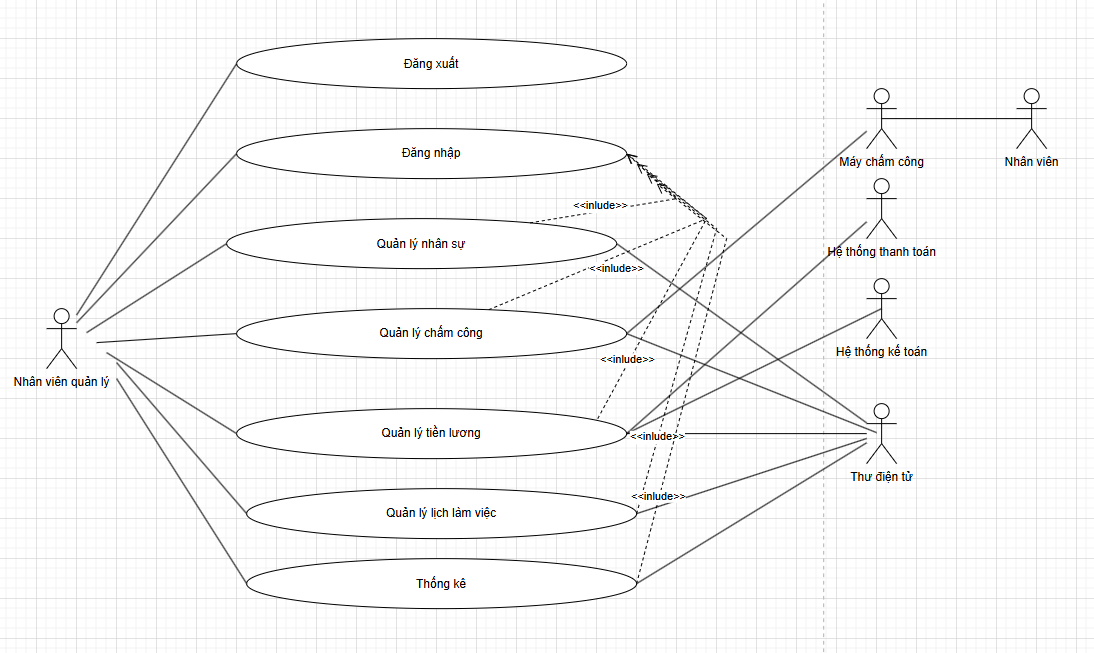
\includegraphics[width=\textwidth]{images/usecase.png}
    \caption{Usecase tổng quát của hệ thống}
    \label{fig:usecase-tong-quat}
\end{figure}

\section{Mô hình xây dựng}
\subsection{Phương án 1: chọn mô hình Scrum}
\begin{itemize}
    \item \textbf{Giới thiệu mô hình:} Scrum là phương pháp phát triển phần mềm linh hoạt theo mô hình Agile, giúp đội dự án có thể thích ứng nhanh với thay đổi từ khách hàng và kiểm soát tiến độ hiệu quả. Scrum được thiết kế để xử lý các dự án có yêu cầu phức tạp, với ít thông tin ban đầu hoặc yêu cầu có thể thay đổi
    \item \textbf{Ưu điểm:}
\begin{itemize}
    \item Dễ dàng thích ứng với thay đổi trong yêu cầu
    \item Có sự cộng tác chặt chẽ giữa các bên
    \item Sản phẩm được phát triển và kiểm thử liên tục, giảm thiểu rủi ro
\end{itemize}
\item \textbf{Nhược điểm:}
\begin{itemize}
    \item Yêu cầu khách hàng tham gia xuyên suốt dự án
    \item Phù hợp với các dự án có yêu cầu linh hoạt, không thích hợp với yêu cầu cố định
\end{itemize}
\end{itemize}
\subsection{Phương án 2: mô hình thác nước (Waterfall)}
\begin{itemize}
    \item \textbf{Giới thiệu mô hình:} Mô hình Thác Nước là quy trình phát triển phần mềm tuyến tính, các giai đoạn được thực hiện tuần tự và không thay đổi khi đã chuyển sang bước tiếp theo
    \item \textbf{Ưu điểm:}
    \begin{itemize}
        \item Quy trình rõ ràng, có thể đo lường tiến độ dự án dễ dàng
        \item Phù hợp với các dự án có yêu cầu cụ thể và cố định từ đầu
        \item Tiết kiệm thời gian và chi phí cho các dự án quy mô nhỏ, ít thay đổi
    \end{itemize}
    \item \textbf{Nhược điểm:} 
    \begin{itemize}
        \item Khó thích ứng với yêu cầu thay đổi của khách hàng trong quá trình phát triển
        \item Lỗi phát hiện ở giai đoạn cuối sẽ tốn kém chi phí và thời gian sửa chữa
        \item Khách hàng chỉ thấy sản phẩm hoàn chỉnh khi kết thúc dự án
    \end{itemize}
\end{itemize}
\subsection{Kết luận về phương án lựa chọn}
\begin{itemize}
    \item Do yêu cầu dự án đã cố định và rõ ràng, quy mô nhỏ: Áp dụng mô hình Thác Nước
    \begin{figure}[H]
        \centering
        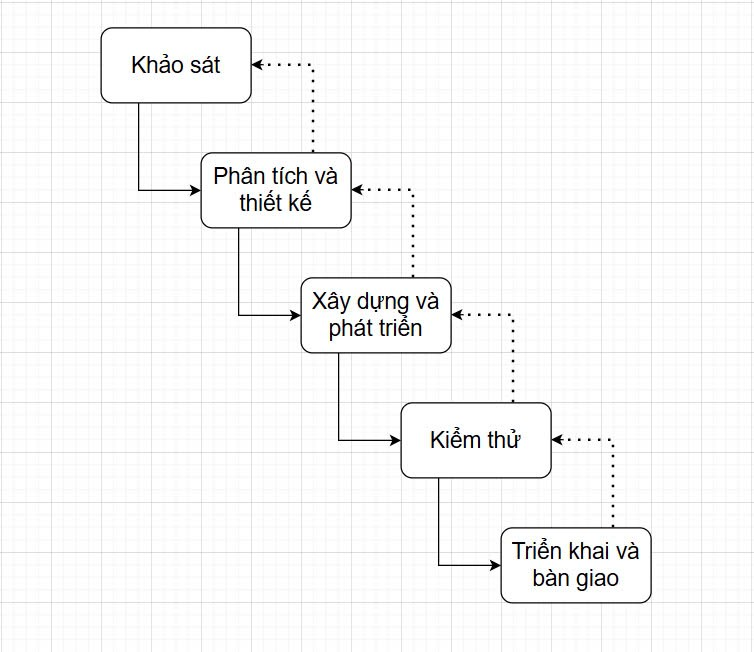
\includegraphics[width=\textwidth]{images/waterfall.png}
        \caption{Mô hình thác nước}
        \label{fig:usecase-tong-quat}
    \end{figure}
\end{itemize}

\section{Phạm vi công việc dự án}
\begin{itemize}
    \item Phạm vi:
\begin{itemize}
    \item Khảo sát
    \item Phân tích và thiết kế
    \item Xây dựng và phát triển hệ thống
    \item Xây dựng và phát triển hệ thống sau kiểm thử
    \item Xây dựng và phát triển hệ thống sau triển khai và chuyển giao
\end{itemize}
\end{itemize}
\begin{itemize}
\item Ngoài phạm vi:
\begin{itemize}
    \item Bảo trì, Nâng cấp
    \item Phát triển hệ thống ở các dạng khác như mobile app, desktop app
\end{itemize}
\end{itemize}

\section{Lịch trình dự án}
\subsection{Khảo sát}
\begin{itemize}
    \item \textbf{Thời gian(5 ngày):} 24/11/2024 - 28/11/2024
    \item \textbf{Công việc:}
    \begin{itemize}
        \item Khảo sát yêu cầu chức năng và phi chức năng (3 ngày): 24/11/2024 - 26/11/2024
        \item Khảo sát quy trình nghiệp vụ (1 ngày): 27/11/2024
        \item Tổng hợp, lập hồ sơ khảo sát (1 ngày): 28/11/2024
    \end{itemize}
    \item \textbf{Thành viên được phân công:} Quang, Phong, Phương, Phát
    \item \textbf{Sản phẩm:} Hồ sơ khảo sát
    \item \textbf{Ước lượng chi phí:} 4.400.000 VND
\end{itemize}
\subsection{Phân tích và thiết kế}
\begin{itemize}
    \item \textbf{Thời gian(13 ngày):}  29/11/2024 - 11/12/2024
    \item \textbf{Công việc:}
    \begin{itemize}
        \item Phân tích quy trình nghiệp vụ (2 ngày): 29/11/2024-30/11/2024
        \item Phân tích yêu cầu (2 ngày): 01/12/2024 - 02/12/2024
        \item TThiết kế kiến trúc hệ thống (2 ngày): 03/12/2024-04/12/2024
        \item Thiết kế CSDL (3 ngày): 05/12/2024 - 07/12/2024
        \item Thiết kế giao diện (4 ngày): 08/12/2024 - 11/12/2024
        \item Lập hồ sơ phân tích thiết kế (1 ngày): 11/12/2024
    \end{itemize}
    \item \textbf{Thành viên được phân công:} Tất cả thành viên
    \item \textbf{Sản phẩm:} Hồ sơ phân tích thiết kế
    \item \textbf{Ước lượng chi phí:} 19.400.000 VND
\end{itemize}
\subsection{Xây dựng và phát triển hệ thống}  
\begin{itemize}
    \item \textbf{Thời gian(17 ngày):} 12/12/2024 - 28/12/2024
    \item \textbf{Công việc:}
    \begin{itemize}
        \item Xây dựng và phát triển CSDL (4 ngày): 12/12/2024 - 15/12/2024
        \item Xây dựng và phát triển Front-end (6 ngày): 16/12/2024 - 21/12/2024
        \item Xây dựng và phát triển Back-end (7 ngày): 22/12/2024 - 28/12/2024
        \item Tích hợp mã nguồn đa tầng (1 ngày): 28/12/2024
    \end{itemize}
    \item \textbf{Thành viên được phân công:} Tất cả thành viên
    \item \textbf{Sản phẩm:} Phần mềm sau tích hợp 
    \item \textbf{Ước lượng chi phí:} 32.400.000 VND
\end{itemize}
\subsection{Xây dựng và phát triển hệ thống sau kiểm thử}
\begin{itemize}
    \item \textbf{Thời gian(8 ngày):} 29/12/2024 - 05/01/2024
    \item \textbf{Công việc:}
    \begin{itemize}
        \item Kiểm thử và sửa lỗi (8 ngày): 29/12/2024 - 05/01/2025 
        \item Lập hồ sơ kiểm thử (1 ngày): 5/01/2025
    \end{itemize}
    \item \textbf{Thành viên được phân công:} Quang,Phát
    \item \textbf{Sản phẩm:} Hồ sơ kiểm thử, Phần mềm sau kiểm thử
    \item \textbf{Ước lượng chi phí:} 4.800.000 VND
\end{itemize}
\subsection{Xây dựng và phát triển hệ thống sau triển khai và chuyển giao}
\begin{itemize}
    \item \textbf{Thời gian(5 ngày):} 06/01/2025 - 10/01/2025
    \item \textbf{Công việc:}
    \begin{itemize}
        \item Viết tài liệu hướng dẫn (1 ngày): 06/01/2025
        \item Chuyển giao cài đặt và Đào tạo sử dụng (2 ngày): 7/1/202025-08/1/2025
        \item Lập hồ sơ triển khai và chuyển giao (2 ngày):  09/01/2025-10/01/2025
    \end{itemize}
    \item \textbf{Thành viên được phân công:} Phương, Hải, Quang
    \item \textbf{Sản phẩm:} Hồ sơ triển khai và bàn giao, Hệ thống sau khi triển khai và chuyển giao
    \item \textbf{Ước lượng chi phí:} 4.600.000 VND
\end{itemize}

\section{Chi phí dự án}
\begin{itemize}
    \item \textbf{Chi phí dự kiến:} 260.000.000 VND
    \item \textbf{Đầu mục chi phí:}
    \begin{itemize}
        \item Tài sản cố định: 15.000.000 VND
        \item Chi phí vận hành: 153.000.000 VND
        \item Chi phí phần mềm: 30.000.000 VND
        \item Phúc lợi và các hoạt động khác: 62.000.000 VND
    \end{itemize}
\end{itemize}

\chapter{Kế hoạch quản lý chi tiết}
\section{Kế hoạch quản lý phạm vi}
\subsection{Phạm vi công việc}
\subsubsection{Phạm vi công việc Khảo sát}
\begin{itemize}
    \item \textbf{Tên Công Việc:} Khảo sát
    \item \textbf{Mô tả công việc:}
    \begin{itemize}
        \item Trao đổi những vấn đề mà doanh nghiệp đang gặp phải trong quá trình quản lý Nhân sự - Tiền lương.
        \item Khảo sát về mong muốn, yêu cầu của doanh nghiệp đối với hệ thống.
        \item Tìm hiểu quy trình quản lý Nhân sự - Tiền lương của doanh nghiệp.
    \end{itemize}
    \item \textbf{Các Sản phẩm của công việc:}
    \begin{itemize}
        \item Báo cáo khảo sát chi tiết
        \item Tài liệu mô tả yêu cầu chức năng và phi chức năng
        \item Tài liệu mô tả quy trình nghiệp vụ
        \item Hồ sơ khảo sát hoàn chỉnh
    \end{itemize}
    \item \textbf{Yêu cầu đánh giá:}
    \begin{itemize}
        \item Báo cáo tài liệu phân tích yêu cầu khách hàng phải rõ ràng và dễ hiểu.
        \item Hoàn thành công việc trong thời gian quy định, không quá 5 ngày.
    \end{itemize}
\end{itemize}
\subsubsection{Phạm vi công việc Khảo sát}
\begin{itemize}
    \item \textbf{Tên Công Việc:} Khảo sát
    \item \textbf{Mô tả công việc:}
    \begin{itemize}
        \item Trao đổi những vấn đề mà doanh nghiệp đang gặp phải trong quá trình quản lý Nhân sự - Tiền lương.
        \item Khảo sát về mong muốn, yêu cầu của doanh nghiệp đối với hệ thống.
        \item Tìm hiểu quy trình quản lý Nhân sự - Tiền lương của doanh nghiệp.
    \end{itemize}
    \item \textbf{Các Sản phẩm của công việc:}
    \begin{itemize}
        \item Báo cáo khảo sát chi tiết
        \item Tài liệu mô tả yêu cầu chức năng và phi chức năng
        \item Tài liệu mô tả quy trình nghiệp vụ
        \item Hồ sơ khảo sát hoàn chỉnh
    \end{itemize}
    \item \textbf{Yêu cầu đánh giá:}
    \begin{itemize}
        \item Báo cáo tài liệu phân tích yêu cầu khách hàng phải rõ ràng và dễ hiểu.
        \item Hoàn thành công việc trong thời gian quy định, không quá 5 ngày.
    \end{itemize}
\end{itemize}

\subsubsection{Phạm vi công việc Phân tích và thiết kế hệ thống}
\begin{itemize}
    \item \textbf{Tên Công Việc:} Phân tích và thiết kế hệ thống
    \item \textbf{Mô tả công việc:}
    \begin{itemize}
        \item Phân tích từ yêu cầu và vấn đề khách hàng thành các yêu cầu cho hệ thống
        \item Thiết kế hệ thống dựa trên kết quả phân tích
    \end{itemize}
    \item \textbf{Các sản phẩm của công việc:}
    \begin{itemize}
        \item Báo cáo phân tích quy trình nghiệp vụ chi tiết cho các phần:
        \begin{itemize}
            \item Quản lý nhân sự
            \item Quản lý phần chấm công
            \item Quản lý hồ sơ tiền lương
            \item Thanh toán lương
        \end{itemize}
        \item Báo cáo phân tích yêu cầu chi tiết cho các phần:
        \begin{itemize}
            \item Yêu cầu giao diện
            \item Yêu cầu chức năng
        \end{itemize}
        \item Các biểu đồ thiết kế hệ thống bao gồm:
        \begin{itemize}
            \item Biểu đồ usecase
            \item Biểu đồ lớp
            \item Biểu đồ tuần tự
            \item Biểu đồ hoạt động
        \end{itemize}
        \item Thiết kế cơ sở dữ liệu chi tiết cho các phần:
        \begin{itemize}
            \item Nhân sự
            \item Hồ sơ lương
            \item Phần chấm công
            \item Thanh toán lương
        \end{itemize}
        \item Các thiết kế giao diện chi tiết cho các phần:
        \begin{itemize}
            \item Quản lý nhân sự
            \item Quản lý hồ sơ lương
            \item Quản lý phần chấm công
            \item Thanh toán lương
        \end{itemize}
        \item Báo cáo tổng hợp và lập bản báo cáo yêu cầu hệ thống
        \item Báo cáo tổng hợp và lập bản báo cáo kiến trúc hệ thống
        \item Báo cáo tổng hợp và lập bản thiết kế giao diện
        \item Hồ sơ phân tích thiết kế
    \end{itemize}
    \item \textbf{Yêu cầu đánh giá:}
    \begin{itemize}
        \item Tài liệu phân tích và thiết kế phải đúng theo tài liệu phân tích yêu cầu khách hàng
        \item Hoàn thành công việc trong thời gian quy định, không quá 15 ngày
    \end{itemize}
\end{itemize}

% \chapter{Thực thi dự án}
\label{Chapter4}
\renewcommand{\arraystretch}{1.2}
\setlength{\LTcapwidth}{\textwidth}
\section{Thực thi giai đoạn Khảo sát}

\fbox{
    \begin{minipage}{\textwidth}
        \begin{center}
            \Large\textbf{BIÊN BẢN NGHIỆM THU CÔNG VIỆC KHẢO SÁT}
        \end{center}
        \vspace{0.1cm}
        \noindent\textbf{TÊN CÔNG VIỆC:} Khảo sát

        \noindent\textbf{Ngày bắt đầu:} 24/11/2024 \\
        \textbf{Ngày kết thúc:} 28/11/2024 \\
        \textbf{Người quản lý:} Hoàng Thu Phương

        \noindent\rule{\textwidth}{0.4pt}

        \noindent\textbf{Ngày nghiệm thu:} 28/11/2024

        \noindent\rule{\textwidth}{0.4pt}

        \noindent\textbf{Sản phẩm công việc đã được nghiệm thu:}
        \begin{enumerate}
            \item Báo cáo khảo sát chi tiết bao gồm:
                  \begin{itemize}
                      \item Các thông tin về đối tượng khảo sát.
                      \item Phương pháp khảo sát.
                      \item Kết quả khảo sát.
                  \end{itemize}
            \item Bảng tổng hợp dữ liệu khảo sát.
            \item Tài liệu hướng dẫn sử dụng kết quả khảo sát cho các mục đích nghiên cứu và phát triển.
        \end{enumerate}
        \noindent\textbf{Tiêu chí nghiệm thu:}
        \begin{itemize}
            \item Báo cáo khảo sát chi tiết, rõ ràng, chính xác.
            \item Bảng tổng hợp dữ liệu đầy đủ, dễ hiểu.
            \item Tài liệu hướng dẫn rõ ràng, áp dụng tốt cho nghiên cứu và phát triển.
        \end{itemize}
    \end{minipage}
}

\fbox{
    \begin{minipage}{\textwidth}
        \noindent\textbf{Quá trình thực hiện:}
        \begin{enumerate}
            \item Xác định mục tiêu và đối tượng khảo sát:
                  \begin{itemize}
                      \item Làm rõ mục đích khảo sát và nhóm đối tượng cần khảo sát.
                  \end{itemize}
            \item Gặp gỡ khách hàng và tiến hành phỏng vấn:
                  \begin{itemize}
                      \item Thu thập thông tin trực tiếp từ khách hàng qua các cuộc họp và phỏng vấn.
                  \end{itemize}
            \item Phân loại thông tin:
                  \begin{itemize}
                      \item Thành yêu cầu chức năng.
                      \item Thành yêu cầu phi chức năng (hiệu suất, bảo mật, khả năng mở rộng).
                  \end{itemize}
            \item Xác định quy trình nghiệp vụ:
                  \begin{itemize}
                      \item Phân tích, mô hình hóa và mô tả chi tiết quy trình nghiệp vụ.
                  \end{itemize}
            \item Tổng hợp và lập hồ sơ khảo sát:
                  \begin{itemize}
                      \item Hệ thống hóa thông tin, xây dựng hồ sơ khảo sát chi tiết.
                  \end{itemize}
        \end{enumerate}

        \noindent\textbf{Thời gian thực hiện:} 5 ngày

        \noindent\textbf{Nguồn lực sử dụng:}
        \begin{itemize}
            \item \textbf{Tài liệu:} Từ các cuộc họp và phỏng vấn khách hàng.
            \item \textbf{Công cụ:} Phần mềm xử lý văn bản, bảng tính (Excel), phần mềm vẽ sơ đồ quy trình.
            \item \textbf{Nhân sự:}
                  \begin{itemize}
                      \item Quang: Khảo sát, ghi nhận thông tin.
                      \item Phong: Khảo sát, ghi nhận thông tin.
                      \item Phương: Tổng hợp và phân tích dữ liệu, lập hồ sơ.
                      \item Phát: Tổng hợp và phân tích dữ liệu, lập hồ sơ.
                  \end{itemize}
        \end{itemize}
        \noindent\textbf{Chi phí:} 4.400.000 VNĐ\\
        \noindent\textbf{Kết quả nghiệm thu:}
        \begin{itemize}
            \item Công việc đã hoàn thành theo đúng yêu cầu và trong thời gian quy định.
            \item Tài liệu và sản phẩm bàn giao đáp ứng đầy đủ tiêu chí chất lượng.
            \item Khách hàng xác nhận hài lòng với kết quả và thanh toán chi phí thực hiện.
        \end{itemize}
        \begin{flushleft}
            \hspace{8cm} \textbf{NGƯỜI THỰC HIỆN} \\
            \hspace{9.5cm} (Ký tên) \\ \vspace{1cm}
        \end{flushleft}
    \end{minipage}
}

%%%
\clearpage
\section{Thực thi giai đoạn Phân tích thiết kế hệ thống}

\fbox{
    \begin{minipage}{\textwidth}
        \begin{center}
            \Large\textbf{BIÊN BẢN NGHIỆM THU CÔNG VIỆC}\\
            \Large\textbf{PHÂN TÍCH THIẾT KẾ HỆ THỐNG}
        \end{center}
        \vspace{0.1cm}
        \noindent\textbf{TÊN CÔNG VIỆC:} Phân tích và thiết kế hệ thống

        \noindent\textbf{Ngày bắt đầu:} 29/11/2024 \\
        \textbf{Ngày kết thúc:} 11/12/2024 \\
        \textbf{Người quản lý:} Hoàng Thu Phương

        \noindent\rule{\textwidth}{0.4pt}

        \noindent\textbf{Ngày nghiệm thu:} 11/12/2024

        \noindent\rule{\textwidth}{0.4pt}

        \noindent\textbf{Sản phẩm công việc đã được nghiệm thu:}
        \begin{enumerate}
            \item Báo cáo phân tích hệ thống chi tiết.
            \item Báo cáo thiết kế hệ thống chi tiết.
            \item Hồ sơ phân tích yêu cầu hệ thống.
            \item Hồ sơ thiết kế hệ thống bao gồm các mô hình, sơ đồ và mô tả chi tiết.
            \item Tài liệu hướng dẫn sử dụng kết quả phân tích và thiết kế cho quá trình phát triển và triển khai.
        \end{enumerate}
        \noindent\textbf{Tiêu chí nghiệm thu:}
        \begin{itemize}
            \item Báo cáo phân tích và thiết kế hệ thống chi tiết, rõ ràng, chính xác.
            \item Hồ sơ phân tích và thiết kế đầy đủ, chi tiết và phân loại rõ ràng.
            \item Tài liệu hướng dẫn rõ ràng, áp dụng tốt cho các bước tiếp theo của quá trình phát triển và triển khai hệ thống.
        \end{itemize}
    \end{minipage}
}
\newpage
\fbox{
    \begin{minipage}{\textwidth}
        \noindent\textbf{Quá trình thực hiện:}
        \begin{enumerate}
            \item Phân tích yêu cầu:
                  \begin{itemize}
                      \item Phân tích các yêu cầu chức năng và phi chức năng của hệ thống.
                  \end{itemize}
            \item Thiết kế hệ thống:
                  \begin{itemize}
                      \item Thiết kế hệ thống bao gồm các mô hình, sơ đồ và mô tả chi tiết.
                  \end{itemize}
            \item Lập báo cáo phân tích và thiết kế:
                  \begin{itemize}
                      \item Lập báo cáo phân tích và thiết kế hệ thống chi tiết.
                  \end{itemize}
            \item Xây dựng hồ sơ phân tích và thiết kế:
                  \begin{itemize}
                      \item Hệ thống hóa toàn bộ thông tin, xây dựng hồ sơ phân tích yêu cầu và thiết kế hệ thống.
                  \end{itemize}
            \item Tạo tài liệu hướng dẫn:
                  \begin{itemize}
                      \item Tạo tài liệu hướng dẫn sử dụng kết quả phân tích và thiết kế cho quá trình phát triển và triển khai.
                  \end{itemize}
        \end{enumerate}

        \noindent\textbf{Thời gian thực hiện:} 13 ngày

        \noindent\textbf{Nguồn lực sử dụng:}
        \begin{itemize}
            \item \textbf{Công cụ:} Phần mềm xử lý văn bản, phần mềm thiết kế hệ thống (như Microsoft Visio, Lucidchart).
            \item \textbf{Nhân lực:}
                  \begin{itemize}
                      \item  Chuyên gia phân tích và thiết kế hệ thống, người lập báo cáo.
                  \end{itemize}
            \item \textbf{Dữ liệu:} Thông tin từ các cuộc họp, phỏng vấn và tài liệu liên quan đến yêu cầu hệ thống.
        \end{itemize}
        \noindent\textbf{Nhân sự:} Cả nhóm: Phân tích thiết kế hệ thống \\
        \noindent\textbf{Chi phí:} 19.400.000 VNĐ \\
        \noindent\textbf{Kết quả nghiệm thu:}
        \begin{itemize}
            \item Công việc đã hoàn thành theo đúng yêu cầu và trong thời gian quy định.
            \item Tài liệu và sản phẩm bàn giao đáp ứng đầy đủ tiêu chí chất lượng.
            \item Khách hàng xác nhận hài lòng với kết quả và thanh toán chi phí thực hiện.
        \end{itemize}

        \begin{flushleft}
            \hspace{8cm} \textbf{NGƯỜI THỰC HIỆN} \\
            \hspace{9.5cm} (Ký tên) \\ \vspace{1cm}
        \end{flushleft}
    \end{minipage}
}

\clearpage
\section{Thực thi giai đoạn Xây dựng và phát triển hệ thống}
\fbox{
    \begin{minipage}{\textwidth}
        \begin{center}
            \Large\textbf{BIÊN BẢN NGHIỆM THU CÔNG VIỆC}\\
            \Large\textbf{XÂY DỰNG VÀ PHÁT TRIỂN HỆ THỐNG}
        \end{center}
        \vspace{0.1cm}
        \noindent\textbf{TÊN CÔNG VIỆC:} Xây dựng và phát triển hệ thống

        \noindent\textbf{Ngày bắt đầu:} 12/12/2024 \\
        \textbf{Ngày kết thúc:} 28/12/2024 \\
        \textbf{Người quản lý:} Hoàng Thu Phương

        \noindent\rule{\textwidth}{0.4pt}

        \noindent\textbf{Ngày nghiệm thu:} 28/12/2024

        \noindent\rule{\textwidth}{0.4pt}

        \noindent\textbf{Sản phẩm công việc đã được nghiệm thu:}
        \begin{itemize}
            \item Hệ thống hoàn chỉnh bao gồm các phần:
                  \begin{itemize}
                      \item Quản lý nhân sự.
                      \item Quản lý hồ sơ lương.
                      \item Quản lý phần chấm công.
                      \item Thanh toán lương.
                      \item Mã nguồn hoàn chỉnh cho việc xây dựng hệ thống (Front-end, Back-end, CSDL).
                      \item Báo cáo chi tiết về quá trình xây dựng và phát triển hệ thống.
                      \item Tài liệu hướng dẫn sử dụng và quản lý hệ thống.
                  \end{itemize}
        \end{itemize}

        \noindent\textbf{Tiêu chí nghiệm thu:}
        \begin{itemize}
            \item Hệ thống phải hoàn chỉnh, không có lỗi và đáp ứng đầy đủ các yêu cầu đã đề ra.
            \item Mã nguồn phải hoàn chỉnh, không có lỗi và đáp ứng đầy đủ các yêu cầu đã đề ra.
            \item Báo cáo chi tiết, rõ ràng và chính xác về quá trình xây dựng và phát triển hệ thống.
            \item Tài liệu hướng dẫn rõ ràng, áp dụng tốt cho các bước tiếp theo của quá trình phát triển và triển khai hệ thống.
        \end{itemize}
    \end{minipage}
}
\newpage
\fbox{
    \begin{minipage}{\textwidth}
        \noindent\textbf{Quá trình thực hiện:}
        \begin{itemize}
            \item Phân tích yêu cầu:
                  \begin{itemize}
                      \item Phân tích các yêu cầu về chức năng và trải nghiệm người dùng (UX).
                  \end{itemize}
            \item Thiết kế hệ thống:
                  \begin{itemize}
                      \item Thiết kế chi tiết, xác định các thành phần và luồng tương tác người dùng.
                  \end{itemize}
            \item Lập trình hệ thống:
                  \begin{itemize}
                      \item Lập trình các phần quản lý nhân sự, hồ sơ lương, chấm công và thanh toán lương theo thiết kế đã đề ra.
                  \end{itemize}
            \item Tổng hợp mã nguồn:
                  \begin{itemize}
                      \item Tổng hợp mã nguồn từ các tầng khác nhau (Front-end, Back-end, CSDL).
                  \end{itemize}
            \item Tích hợp mã nguồn:
                  \begin{itemize}
                      \item Tích hợp các thành phần của hệ thống thành một tổng thể hoàn chỉnh.
                  \end{itemize}
            \item Kiểm tra và xác nhận:
                  \begin{itemize}
                      \item Kiểm tra và xác nhận hệ thống sau khi tích hợp để đảm bảo không có lỗi.
                  \end{itemize}
            \item Lập báo cáo:
                  \begin{itemize}
                      \item Lập báo cáo chi tiết về quá trình xây dựng và phát triển hệ thống.
                  \end{itemize}
            \item Tạo tài liệu hướng dẫn:
                  \begin{itemize}
                      \item Tạo tài liệu hướng dẫn sử dụng và quản lý hệ thống.
                  \end{itemize}
        \end{itemize}

        \noindent\textbf{Thời gian thực hiện:} 16 ngày

        \noindent\textbf{Nguồn lực sử dụng:}
        \begin{itemize}
            \item Công cụ:
                  \begin{itemize}
                      \item Phần mềm thiết kế và lập trình giao diện (Adobe XD, Figma, HTML, CSS, JavaScript).
                      \item Phần mềm lập trình Back-end (Visual Studio Code, IntelliJ IDEA).
                      \item Phần mềm quản lý mã nguồn (Git).
                      \item Công cụ CI/CD (Jenkins, GitLab CI).
                      \item Phần mềm xử lý văn bản.
                  \end{itemize}
            \item Nhân lực:
                  \begin{itemize}
                      \item Chuyên gia lập trình Front-end, Back-end, CSDL, người lập báo cáo.
                  \end{itemize}
            \item Dữ liệu:
                  \begin{itemize}
                      \item Thông tin từ các cuộc họp, phỏng vấn và tài liệu liên quan đến yêu cầu hệ thống.
                  \end{itemize}
        \end{itemize}

        \noindent\textbf{Nhân sự:} Cả nhóm: Xây dựng và phát triển hệ thống \\
        \noindent\textbf{Chi phí:} 32.400.000 VNĐ \\
    \end{minipage}
}
\newpage
\fbox{
    \begin{minipage}{\textwidth}
        \noindent\textbf{Kết quả nghiệm thu:}
        \begin{itemize}
            \item Công việc đã hoàn thành theo đúng yêu cầu và trong thời gian quy định.
            \item Hệ thống hoàn chỉnh, mã nguồn và tài liệu bàn giao đáp ứng đầy đủ tiêu chí chất lượng.
            \item Khách hàng xác nhận hài lòng với kết quả và thanh toán chi phí thực hiện.
        \end{itemize}

        \begin{flushleft}
            \hspace{8cm} \textbf{NGƯỜI THỰC HIỆN} \\
            \hspace{9.5cm} (Ký tên) \\ \vspace{1cm}
        \end{flushleft}

    \end{minipage} \\
}
%%%
\section{Thực thi giai đoạn Xây dựng và phát triển hệ thống sau kiểm thử}

\fbox{
    \begin{minipage}{\textwidth}
        \begin{center}
            \Large\textbf{BIÊN BẢN NGHIỆM THU CÔNG VIỆC}\\
            \Large\textbf{XÂY DỰNG VÀ PHÁT TRIỂN HỆ THỐNG SAU KIỂM THỬ}
        \end{center}
        \vspace{0.1cm}
        \noindent\textbf{TÊN CÔNG VIỆC:} Xây dựng và phát triển hệ thống

        \noindent\textbf{Ngày bắt đầu:} 29/12/2024 \\
        \textbf{Ngày kết thúc:} 05/01/2024 \\
        \textbf{Người quản lý:} Hoàng Thu Phương

        \noindent\rule{\textwidth}{0.4pt}

        \noindent\textbf{Ngày nghiệm thu:} 05/01/2024

        \noindent\rule{\textwidth}{0.4pt}

        \noindent\textbf{Sản phẩm công việc đã được nghiệm thu:}
        \begin{itemize}
            \item Hệ thống hoàn chỉnh sau kiểm thử và bao gồm:
                  \begin{itemize}
                      \item Hồ sơ kiểm thử hoàn chỉnh.
                      \item Kết quả chạy testcase.
                      \item Báo cáo kiểm tra và sửa lỗi.
                      \item Báo cáo chi tiết về quá trình kiểm thử và sửa lỗi.
                      \item Tài liệu hướng dẫn sử dụng và quản lý phần mềm sau kiểm thử.
                  \end{itemize}
        \end{itemize}
    \end{minipage} \\
}

\newpage
\fbox{
    \begin{minipage}{\textwidth}
        \noindent\textbf{Tiêu chí nghiệm thu:}
        \begin{itemize}
            \item Phần mềm phải hoàn chỉnh, không có lỗi và đáp ứng đầy đủ các yêu cầu đã đề ra.
            \item Hồ sơ kiểm thử phải đầy đủ, chi tiết và bao phủ tất cả các chức năng của hệ thống.
            \item Báo cáo chi tiết, rõ ràng và chính xác về quá trình kiểm thử và sửa lỗi.
            \item Tài liệu hướng dẫn rõ ràng, dễ hiểu và áp dụng tốt cho các bước tiếp theo của quá trình quản lý và sử dụng phần mềm.
        \end{itemize}
        \noindent\textbf{Quá trình thực hiện:}
        \begin{itemize}
            \item Ghi nhận kết quả:
                  \begin{itemize}
                      \item Ghi nhận kết quả chạy testcase, bao gồm các lỗi phát hiện được.
                  \end{itemize}
            \item Phân tích kết quả:
                  \begin{itemize}
                      \item Phân tích kết quả chạy testcase để xác định các vấn đề cần khắc phục.
                  \end{itemize}
            \item Kiểm tra và sửa lỗi:
                  \begin{itemize}
                      \item Thực hiện kiểm tra và sửa lỗi trong hệ thống theo thứ tự ưu tiên.
                  \end{itemize}
            \item Kiểm tra lại:
                  \begin{itemize}
                      \item Kiểm tra lại hệ thống sau khi sửa lỗi để đảm bảo lỗi đã được khắc phục hoàn toàn.
                  \end{itemize}
            \item Lập báo cáo:
                  \begin{itemize}
                      \item Lập báo cáo chi tiết về quá trình kiểm thử và sửa lỗi.
                  \end{itemize}
            \item Tạo tài liệu hướng dẫn:
                  \begin{itemize}
                      \item Tạo tài liệu hướng dẫn sử dụng và quản lý phần mềm sau kiểm thử.
                  \end{itemize}
        \end{itemize}

        \noindent\textbf{Thời gian thực hiện:} 8 ngày

        \noindent\textbf{Nguồn lực sử dụng:}
        \begin{itemize}
            \item Công cụ:
                  \begin{itemize}
                      \item Phần mềm quản lý kiểm thử (TestRail, JIRA).
                      \item Phần mềm kiểm thử tự động (nếu có).
                      \item Phần mềm quản lý lỗi (JIRA, Bugzilla).
                      \item Phần mềm lập trình (Visual Studio Code, IntelliJ IDEA).
                      \item Phần mềm xử lý văn bản.
                  \end{itemize}
            \item Nhân lực:
                  \begin{itemize}
                      \item Chuyên gia kiểm thử, lập trình viên, người lập báo cáo.
                  \end{itemize}
            \item Dữ liệu:
                  \begin{itemize}
                      \item Thông tin từ các cuộc họp, phỏng vấn và tài liệu liên quan đến yêu cầu kiểm thử hệ thống.
                  \end{itemize}
        \end{itemize}

        \noindent\textbf{Nhân sự:} Cả nhóm: Xây dựng và phát triển hệ thống sau kiểm thử \\
        \noindent\textbf{Chi phí:} 4.800.000 VNĐ \\

    \end{minipage} \\
}
\newpage
\fbox{
    \begin{minipage}{\textwidth}
        \noindent\textbf{Kết quả nghiệm thu:}
        \begin{itemize}
            \item Công việc đã hoàn thành theo đúng yêu cầu và trong thời gian quy định.
            \item Phần mềm, hồ sơ kiểm thử, báo cáo và tài liệu bàn giao đáp ứng đầy đủ tiêu chí chất lượng.
            \item Khách hàng xác nhận hài lòng với kết quả và thanh toán chi phí thực hiện.
        \end{itemize}

        \begin{flushleft}
            \hspace{8cm} \textbf{NGƯỜI THỰC HIỆN} \\
            \hspace{9.5cm} (Ký tên) \\ \vspace{1cm}
        \end{flushleft}

    \end{minipage} \\
}
%%%
\section{Thực thi giai đoạn Xây dựng và phát triển hệ thống sau triển khai và chuyển giao}
\fbox{
    \begin{minipage}{\textwidth}
        \begin{center}
            \Large\textbf{BIÊN BẢN NGHIỆM THU CÔNG VIỆC}\\
            \Large\textbf{XÂY DỰNG VÀ PHÁT TRIỂN HỆ THỐNG SAU KIỂM THỬ}
        \end{center}
        \vspace{0.1cm}
        \noindent\textbf{TÊN CÔNG VIỆC:} Xây dựng và phát triển hệ thống

        \noindent\textbf{Ngày bắt đầu:} 06/01/2024 \\
        \textbf{Ngày kết thúc:} 10/01/2024 \\
        \textbf{Người quản lý:} Hoàng Thu Phương

        \noindent\rule{\textwidth}{0.4pt}

        \noindent\textbf{Ngày nghiệm thu:} 10/01/2024

        \noindent\rule{\textwidth}{0.4pt}

        \noindent\textbf{Sản phẩm công việc đã được nghiệm thu:}
        \begin{itemize}
            \item Hệ thống hoàn chỉnh sau kiểm thử và bao gồm:
                  \begin{itemize}
                      \item Hồ sơ triển khai và chuyển giao hoàn chỉnh.
                      \item Tài liệu hướng dẫn sử dụng.
                      \item Báo cáo chi tiết về quá trình bàn giao và cài đặt.
                      \item Báo cáo chi tiết về quá trình đào tạo và sử dụng.
                      \item Báo cáo chi tiết về quá trình chuyển giao.
                      \item Tài liệu hướng dẫn sử dụng và quản lý hệ thống sau khi chuyển giao.
                  \end{itemize}
        \end{itemize}
    \end{minipage} \\
}

\newpage
\fbox{
    \begin{minipage}{\textwidth}
        \noindent\textbf{Tiêu chí nghiệm thu:}
        \begin{itemize}
            \item Phần mềm phải hoàn chỉnh, không có lỗi và đáp ứng đầy đủ các yêu cầu đã đề ra.
            \item Hồ sơ triển khai và chuyển giao phải đầy đủ, chi tiết và bao phủ tất cả các bước cần thiết.
            \item Báo cáo phải chi tiết, rõ ràng và chính xác về quá trình chuyển giao.
            \item Tài liệu hướng dẫn phải dễ hiểu và có thể áp dụng cho các bước tiếp theo của quá trình quản lý và sử dụng hệ thống.
        \end{itemize}
        \noindent\textbf{Quá trình thực hiện:}
        \begin{itemize}
            \item Giám sát và bảo trì hệ thống:
                  \begin{itemize}
                      \item Theo dõi hoạt động của phần mềm để phát hiện và xử lý kịp thời các sự cố.
                      \item Thực hiện các công việc bảo trì định kỳ để đảm bảo phần mềm hoạt động ổn định.
                  \end{itemize}
            \item  Hỗ trợ người dùng:
                  \begin{itemize}
                      \item Cung cấp hỗ trợ kỹ thuật cho người dùng trong quá trình sử dụng phần mềm.
                      \item Giải đáp các thắc mắc và hướng dẫn người dùng về các chức năng của phần mềm.
                  \end{itemize}
            \item Khắc phục sự cố:
                  \begin{itemize}
                      \item Xử lý các lỗi phát sinh trong quá trình sử dụng phần mềm.
                      \item Cập nhật và vá lỗi phần mềm để đảm bảo tính ổn định và bảo mật.
                  \end{itemize}
            \item  Cải tiến phần mềm:
                  \begin{itemize}
                      \item Thu thập phản hồi từ người dùng để cải tiến và nâng cao chất lượng phần mềm.
                      \item Thực hiện các thay đổi và cập nhật phần mềm dựa trên yêu cầu của người dùng và quản lý.
                  \end{itemize}
            \item Lập báo cáo:
                  \begin{itemize}
                      \item Lập báo cáo chi tiết về tình trạng hoạt động của phần mềm sau khi chuyển giao.
                      \item Báo cáo về các sự cố đã xử lý và các cải tiến đã thực hiện.
                  \end{itemize}
        \end{itemize}

        \noindent\textbf{Thời gian thực hiện:} 6 ngày

        \noindent\textbf{Nguồn lực sử dụng:}
        \begin{itemize}
            \item Công cụ:
                  \begin{itemize}
                      \item Phần mềm giám sát hệ thống (Nagios, Zabbix).
                      \item Phần mềm quản lý lỗi (JIRA, Bugzilla).
                      \item Phần mềm xử lý văn bản.
                  \end{itemize}
            \item Nhân lực:
                  \begin{itemize}
                      \item Chuyên gia hỗ trợ kỹ thuật, lập trình viên, người lập báo cáo.
                  \end{itemize}
            \item Dữ liệu:
                  \begin{itemize}
                      \item Thông tin từ các cuộc họp, phản hồi của người dùng và tài liệu liên quan đến phần mềm.
                  \end{itemize}
        \end{itemize}
    \end{minipage} \\
}
\newpage
\fbox{
    \begin{minipage}{\textwidth}
        \noindent\textbf{Nhân sự:} Cả nhóm: Xây dựng và phát triển hệ thống sau triển khai và chuyển giao \\
        \noindent\textbf{Chi phí:} 4.600.000 VNĐ \\
        \noindent\textbf{Kết quả nghiệm thu:}
        \begin{itemize}
            \item Công việc đã hoàn thành theo đúng yêu cầu và trong thời gian quy định.
            \item Phần mềm, hồ sơ kiểm thử, báo cáo và tài liệu bàn giao đáp ứng đầy đủ tiêu chí chất lượng.
            \item Khách hàng xác nhận hài lòng với kết quả và thanh toán chi phí thực hiện.
        \end{itemize}

        \begin{flushleft}
            \hspace{8cm} \textbf{NGƯỜI THỰC HIỆN} \\
            \hspace{9.5cm} (Ký tên) \\ \vspace{1cm}
        \end{flushleft}

    \end{minipage} \\
}

% \chapter{Kết thúc dự án}
\label{Chapter5}

\section{Biên bản kết thúc dự án}
\fbox{
    \begin{minipage}{\textwidth}
        \begin{center}
            \Large\textbf{BIÊN BẢN KẾT THÚC DỰ ÁN}
        \end{center}
        \vspace{0.2cm}
        \noindent\textbf{Tên dự án:} Xây dựng và phát triển hệ thống thông tin quản lý Nhân sự - Tiền lương

        \noindent\textbf{Thời gian thực hiện dự án:} 24/11/2024 đến 22/01/2025 \\
        \textbf{Bên A - Nhà đầu tư:} Công ty bất động sản Vinhome \\
        \textbf{Bên B - Giám đốc dự án:} Hoàng Thu Phương (Người đại diện)

        \noindent\rule{\textwidth}{0.4pt}

        \noindent\textbf{1. Mục đích biên bản}
        \begin{itemize}
            \item Ghi nhận việc kết thúc dự án đã hoàn thành theo kế hoạch.
            \item Xác nhận các sản phẩm chuyển giao đã đạt được yêu cầu và mục tiêu ban đầu.
            \item Đề xuất các khuyến nghị hoặc kinh nghiệm cho các dự án trong tương lai.
        \end{itemize}

        \noindent\textbf{2. Các sản phẩm chuyển giao}\\
        \begin{tabular}{|c|p{0.5\textwidth}|c|c|}
            \hline
            \textbf{STT} & \textbf{Sản phẩm}                                    & \textbf{Thời gian bàn giao} & \textbf{Trạng thái} \\ \hline
            1            & Hồ sơ khảo sát                                       & 28/11/2024                  & Hoàn thành          \\ \hline
            2            & Hồ sơ phân tích và thiết kế                          & 13/12/2024                  & Hoàn thành          \\ \hline
            3            & Phần mềm sau tích hợp                                & 07/01/2025                  & Hoàn thành          \\ \hline
            4            & Hồ sơ kiểm thử, Phần mềm sau kiểm thử                & 14/01/2025                  & Hoàn thành          \\ \hline
            5            & Hồ sơ triển khai và chuyển giao, Phần mềm hoàn thiện & 22/01/2025                  & Hoàn thành          \\ \hline
        \end{tabular}     
	\end{minipage}
}
\newpage
\fbox{
    \begin{minipage}{\textwidth}
        \noindent\textbf{3. Kết quả đạt được}
        \begin{itemize}
            \item Yêu cầu chức năng: Hệ thống đã đảm bảo các chức năng cần thiết như:
                  \begin{itemize}
                      \item Quản lý nhân sự, Quản lý chấm công, Quản lý lương, Quản lý lịch làm việc
                      \item Xem lương, xem lịch làm việc, chấm công.
                  \end{itemize}
            \item Yêu cầu phi chức năng:
                  \begin{itemize}
                      \item Giao diện thân thiện, đẹp, dễ sử dụng.
                      \item Hệ thống được tích hợp mượt mà, hoạt động ổn định.
                      \item Khả năng mở rộng dễ dàng.
                  \end{itemize}
        \end{itemize}
        \vspace{0.5cm}

        \noindent\textbf{4. Các hoạt động kết thúc dự án}
        \begin{table}[H]
            \centering
            \begin{tabular}{|c|p{0.3\textwidth}|p{0.3\textwidth}|}
                \hline
                \textbf{Hoạt động}     & \textbf{Người thực hiện}     & \textbf{Trách nhiệm}                                               \\ \hline
                Đánh giá kết quả dự án & Trưởng nhóm Hoàng Thu Phương & Đánh giá tính hoàn thiện của sản phẩm dựa trên yêu cầu ban đầu.    \\ \hline
                Xác nhận bàn giao      & Công ty Vinhome              & Xác nhận hệ thống hoạt động đúng yêu cầu.                          \\ \hline
                Lập biên bản kết thúc  & Các bên tham gia             & Ghi nhận các kết quả đạt được, kinh nghiệm và khuyến nghị.         \\ \hline
                Bàn giao chính thức    & Các bên tham gia             & Hoàn thành việc bàn giao, đảm bảo không có tranh chấp về sản phẩm. \\ \hline
            \end{tabular}
        \end{table}

        \vspace{0.5cm}

        \noindent\textbf{5. Ràng buộc được đáp ứng}
        \begin{itemize}
            \item \textbf{Tiến độ:} Dự án đã hoàn thành đúng thời hạn như thỏa thuận (22/01/2025).
            \item \textbf{Ngân sách:} Tổng chi phí dự án không vượt quá ngân sách đã phê duyệt.
            \item \textbf{Tương thích:} Hệ thống được phát triển tương thích với cơ sở hạ tầng hiện tại của công ty bất động sản Vinhome.
            \item \textbf{Yêu cầu kỹ thuật:} Đáp ứng đầy đủ các tiêu chí về giao diện, hiệu suất và khả năng mở rộng.
        \end{itemize}

        \vspace{0.5cm}

        \noindent\textbf{6. Xác nhận kết thúc}
        Chúng tôi, các bên tham gia, đã xem xét và đồng ý rằng dự án đã hoàn thành đúng mục tiêu và yêu cầu ban đầu. Không có tranh chấp nào liên quan đến sản phẩm chuyển giao.
        \noindent\rule{\textwidth}{0.4pt}
        \begin{flushright}
            \textbf{Hà Nội, ngày ... tháng ... năm 2025} \\ \vspace{0.5cm}
        \end{flushright}
        \begin{flushleft}
            \hspace{2cm} \textbf{Bên A} \hspace{6cm} \textbf{Bên B}\\
            \hspace{1cm} Đại diện: Công ty Vinhome \hspace{3.5cm} Đại diện: Hoàng Thu Phương\\
            \hspace{2cm} Ký tên          \hspace{6cm} Ký tên\\ \vspace{1cm}
        \end{flushleft}
	\end{minipage}
}        

\section{Biên bản thanh lý hợp đồng}
\fbox{
    \begin{minipage}{\textwidth}
        \begin{center}
            \Large\textbf{BIÊN BẢN THANH LÝ HỢP ĐỒNG}
        \end{center}
        \vspace{0.2cm}
        \noindent\textbf{Căn cứ:} Xây dựng và phát triển hệ thống thông tin quản lý Nhân sự - Tiền lương

        \begin{itemize}
            \item Hợp đồng số: 88/2024/HĐKD đã ký ngày …/…/2024 giữa Công ty Bất động sản Vinhome (Bên A) và Hoàng Thu Phương (Bên B).
            \item Biên bản kết thúc dự án “Xây dựng và phát triển hệ thống thông tin quản lý nhân sự - tiền lương” ngày 22/01/2025.
        \end{itemize}

        \noindent\textbf{Hôm nay, ngày 22 tháng 01 năm 2025} , tại văn phòng Công ty Bất động sản Vinhome, chúng tôi gồm:

        \noindent\textbf{1. Bên A - Nhà đầu tư:} Công ty Bất động sản Vinhome
        \begin{itemize}
            \item Đại diện: Nguyễn Xuân Sơn
            \item Chức vụ: Giám đốc điều hành Công ty Bất động sản Vinhome
            \item Địa chỉ: 18 Đa Tống
            \item Điện thoại: 123456789
            \item Email: nguyenxuanson@gmail.com
        \end{itemize}
        \noindent\textbf{2. Bên B - Đơn vị thực hiện dự án:} Hoàng Thu Phương
        \begin{itemize}
            \item Đại diện: Hoàng Thu Phương
            \item Chức vụ: Giám đốc dự án
            \item Địa chỉ: 175 Tây Sơn
            \item Điện thoại: 123456789
            \item Email: phuongthuhoang@gmail.com
        \end{itemize}
	\end{minipage}
}
\newpage
\fbox{
    \begin{minipage}{\textwidth}
        \noindent\textbf{1. Nội dung thanh lý hợp đồng} \\
        \noindent\textbf{1.1 Hai bên xác nhận rằng:}
        \begin{itemize}
            \item Bên B đã hoàn thành toàn bộ các nghĩa vụ theo hợp đồng số …/2024/HĐKD, bao gồm việc bàn giao các sản phẩm theo đúng chất lượng và tiến độ đã cam kết.
            \item Bên A đã nhận đủ các sản phẩm từ Bên B và xác nhận rằng các sản phẩm này đáp ứng đầy đủ yêu cầu được ghi trong hợp đồng
        \end{itemize}
        \noindent\textbf{1.2. Các sản phẩm chuyển giao}
        \begin{itemize}
            \item Hợp đồng số 88/2024/HĐKD chính thức được thanh lý từ ngày 22/01/2025.
            \item Sau thời điểm này, hai bên không còn nghĩa vụ pháp lý hay tài chính nào liên quan đến hợp đồng trên, ngoại trừ các trách nhiệm bảo hành (nếu có) được nêu trong hợp đồng.
        \end{itemize}
        \noindent\rule{\textwidth}{0.4pt}

        \vspace{0.2cm}

        \noindent\textbf{2. Các khoản thanh toán} \\
        \noindent\textbf{2.1. Tổng giá trị hợp đồng:} 260.000.000 VNĐ.
        \noindent\textbf{2.2. Khoản đã thanh toán:}
        \begin{itemize}
            \item 20\% giá trị hợp đồng: 52.000.000 VNĐ (đã thanh toán ngày 28/11/2024).
            \item 20\% giá trị hợp đồng: 52.000.000 VNĐ (đã thanh toán ngày 13/12/2024).
            \item 20\% giá trị hợp đồng: 52.000.000 VNĐ (đã thanh toán ngày 07/01/2024).
            \item 20\% giá trị hợp đồng: 52.000.000 VNĐ (đã thanh toán ngày 14/01/2024).
            \item 20\% giá trị còn lại: 52.000.000 VNĐ (được thanh toán sau khi bàn giao đầy đủ sản phẩm ngày 22/01/2025).
        \end{itemize}
        \noindent\textbf{2.3. Xác nhận thanh toán:}
        \begin{itemize}
            \item Bên B xác nhận đã nhận đủ tổng giá trị hợp đồng là 260.000.000 VNĐ từ Bên A.
        \end{itemize}

        \noindent\rule{\textwidth}{0.4pt}

        \noindent\textbf{3. Cam kết của các bên}
        \begin{itemize}
            \item Hai bên cam kết thực hiện đúng nội dung biên bản thanh lý hợp đồng này.
            \item Biên bản được lập thành 02 bản, mỗi bên giữ 01 bản và có giá trị pháp lý như nhau.
        \end{itemize}
        \noindent\rule{\textwidth}{0.4pt}
        \begin{flushright}
            \textbf{Hà Nội, ngày ... tháng ... năm 2025} \\ \vspace{0.5cm}
        \end{flushright}
        \begin{flushleft}
            \hspace{2cm} \textbf{Bên A} \hspace{8cm} \textbf{Bên B}\\
            \hspace{1cm} Đại diện: Công ty Vinhome \hspace{3.5cm} Đại diện: Hoàng Thu Phương\\
            \hspace{2cm} Ký tên          \hspace{8cm} Ký tên\\ \vspace{1cm}
        \end{flushleft}
	\end{minipage}
}


% Công trình của tác giả (nếu không có thì comment 02 dòng dưới)
\addcontentsline{toc}{chapter}{Danh mục công trình của tác giả}
\chapter*{Danh mục công trình của tác giả}
\label{Appendix1}

\begin{enumerate}
\item Le, Viet-Tuan and Kim, Yong-Guk. “Attention-based residual autoencoder for video anomaly
detection”. In: Applied Intelligence 53.3 (2023), pp. 3240–3254. issn: 1573-7497. doi: \url{https://doi.org/10.1007/s10489-022-03613-1}.

\end{enumerate}

% In tài liệu tham khảo
\addcontentsline{toc}{chapter}{Tài liệu tham khảo}
\printbibheading[title={Tài liệu tham khảo}]

%\printbibliography[heading=subbibliography, title={Tiếng Việt}, keyword=\textbf{Tieng}, resetnumbers=true]

\DeclareNameAlias{sortname}{last-first}
\DeclareNameAlias{default}{last-first}

\printbibliography[heading=subbibliography, title={Tiếng Anh}, notkeyword=Tieng, resetnumbers=1] 
% ===================================================================== %
% CHÚ Ý: phải gán lại resetnumbers=số tài liệu tham khảo tiếng Việt + 1 %
% ===================================================================== %

% Phần phụ lục
\appendix

\chapter{Tên phụ lục 1}
\label{Appendix1}

Đây là phụ lục.

\end{document} 